% ==========================================
% step04.tex
% ==========================================
\section{بخش چهارم: بهبود کیفیت با گاما کرکشن (تبدیلات توانی)}

\noindent
تبدیلات خطی (مانند انتقال افاین) هیستوگرام را به صورت یکنواخت در تمام طیف‌ها می‌کشند که منجر به از دست رفتن اطلاعات در کرانه‌ها (\lr{Clipping}) می‌شود. در مقابل، تبدیلات توانی یک نگاشت غیرخطی ارائه می‌دهند که فرمول پایه آن $s = c r^\gamma$ است. 

\begin{stepbox}
\field{۱. تحلیل رفتار ریاضی مقادیر مختلف $\gamma$}{
رفتار تابع توانی مستقیماً به مقدار $\gamma$ بستگی دارد. به طور مرسوم مقدار ثابت $c = 1$ در نظر گرفته می‌شود:
\begin{itemize}[leftmargin=*]
    \item \textbf{توان‌های کسری ($\gamma < 1$):} دامنه باریکی از مقادیر تاریک ورودی را به بازه وسیع‌تری از مقادیر خروجی نگاشت می‌کنند. این مقادیر برای تصویر \texttt{DarkImage} که نیاز به باز شدن بافت‌های تاریک دارد، ایده‌آل هستند و همزمان از سفیدسوختگی نواحی روشن جلوگیری می‌کنند.
    \item \textbf{توان‌های بزرگتر از یک ($\gamma > 1$):} اثری کاملاً معکوس نسبت به توان‌های کسری دارند. اعمال این مقادیر بر روی تصویر \texttt{BrightImage}، رنگ‌پریدگی تصویر را با فشرده‌سازی مقادیر روشن و کشیدن مقادیر تاریک‌تر جبران می‌کند.
\end{itemize}
}
\end{stepbox}

\begin{warnbox}[اهمیت حیاتی نرمال‌سازی در گاما کُرکشن]
همان‌طور که در بررسی‌های اولیه مشخص شد، اعمال مستقیم توان بر روی مقادیر $[0, 255]$ منجر به تولید اعداد نجومی و اشباع شدن تصویر می‌شود. برای پیاده‌سازی اصولی، ابتدا باید تصویر به بازه پیوسته $[0, 1]$ نرمال‌سازی شود. پس از اعمال توان، از آنجا که به توان رساندن اعداد بین صفر و یک، آن‌ها را از این بازه خارج نمی‌کند، محاسبات بدون خطا انجام شده و در نهایت با ضرب در ۲۵۵ به مقیاس \texttt{uint8} بازگردانده می‌شود.
\end{warnbox}
\newpage
\begin{codebox}[پیاده‌سازی اصولی الگوریتم گاما کُرکشن با نرمال‌سازی]
\begin{lstlisting}[language=Python]
gammas = [1, 0.8, 0.9, 1.1, 1.2]

for m in gammas:
    # 1. Normalize to [0, 1] using float32 to prevent overflow
    I_DI_norm = I_DI.astype(np.float32) / 255.0
    I_BI_norm = I_BI.astype(np.float32) / 255.0
    
    # 2. Apply Power-law transformation (s = c * r^gamma, where c=1)
    I_DI_gamma = I_DI_norm ** m
    I_BI_gamma = I_BI_norm ** m
    
    # 3. Scale back to [0, 255] and cast to uint8
    processed_DI = np.clip(I_DI_gamma * 255.0, 0, 255).astype(np.uint8)
    processed_BI = np.clip(I_BI_gamma * 255.0, 0, 255).astype(np.uint8)
\end{lstlisting}
\end{codebox}

\begin{figure}[htbp]
\centering
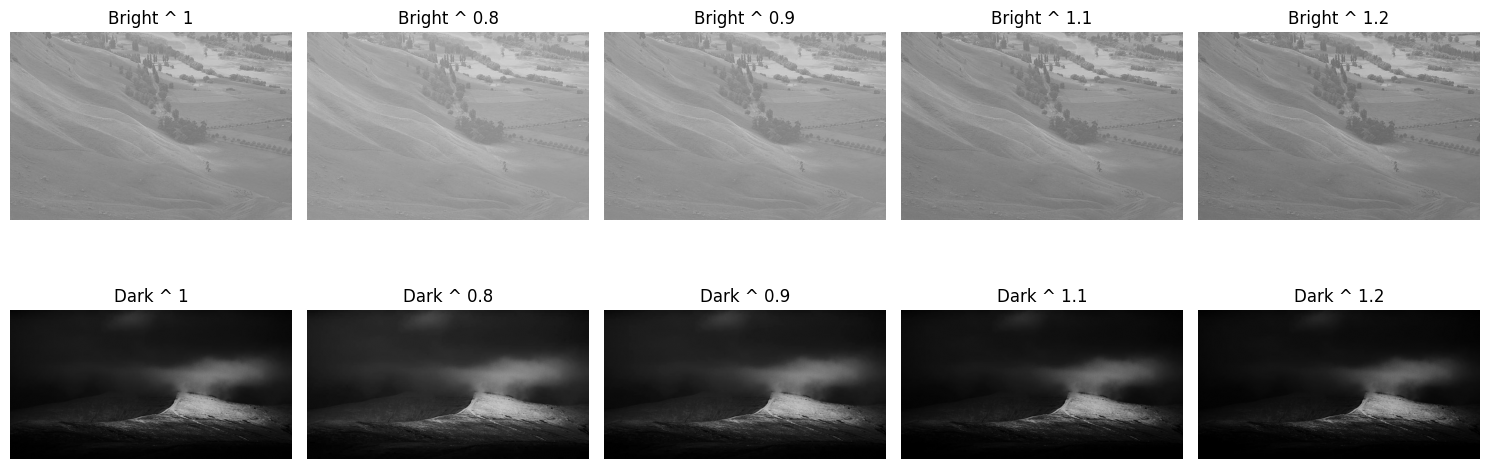
\includegraphics[width=\textwidth]{images/image_24a45c.png}
\caption{نتایج اعمال گاما کرکشن. توان‌های کسری (سمت چپ) جزئیات تاریک کوهستان را در \texttt{DarkImage} به زیبایی نمایان کرده‌اند و توان‌های بزرگتر از یک (سمت راست) کنتراست \texttt{BrightImage} را بازگردانده‌اند.}
\label{fig:gamma_visual_correct}
\end{figure}

\begin{stepbox}
\field{۲. تحلیل هیستوگرام‌ها و مزیت نگاشت غیرخطی}{
با دقت در هیستوگرام‌های خروجی، تفاوت اصلی این روش با انتقال افاین آشکار می‌شود. به دلیل استفاده از نرمال‌سازی و ذات غیرخطی تابع توانی، هیچ قله‌ی مصنوعی (\lr{Spike}) در مقادیر ۰ و ۲۵۵ ایجاد نشده است. تابع گاما به جای برش دادن اطلاعات (\lr{Clipping})، توزیع پیکسل‌ها را به صورت نرم (\lr{Smooth}) فشرده یا بسط داده و تمام جزئیات تصویر را در هر دو کرانه نوری حفظ کرده است.
}
\end{stepbox}

\begin{figure}[htbp]
\centering
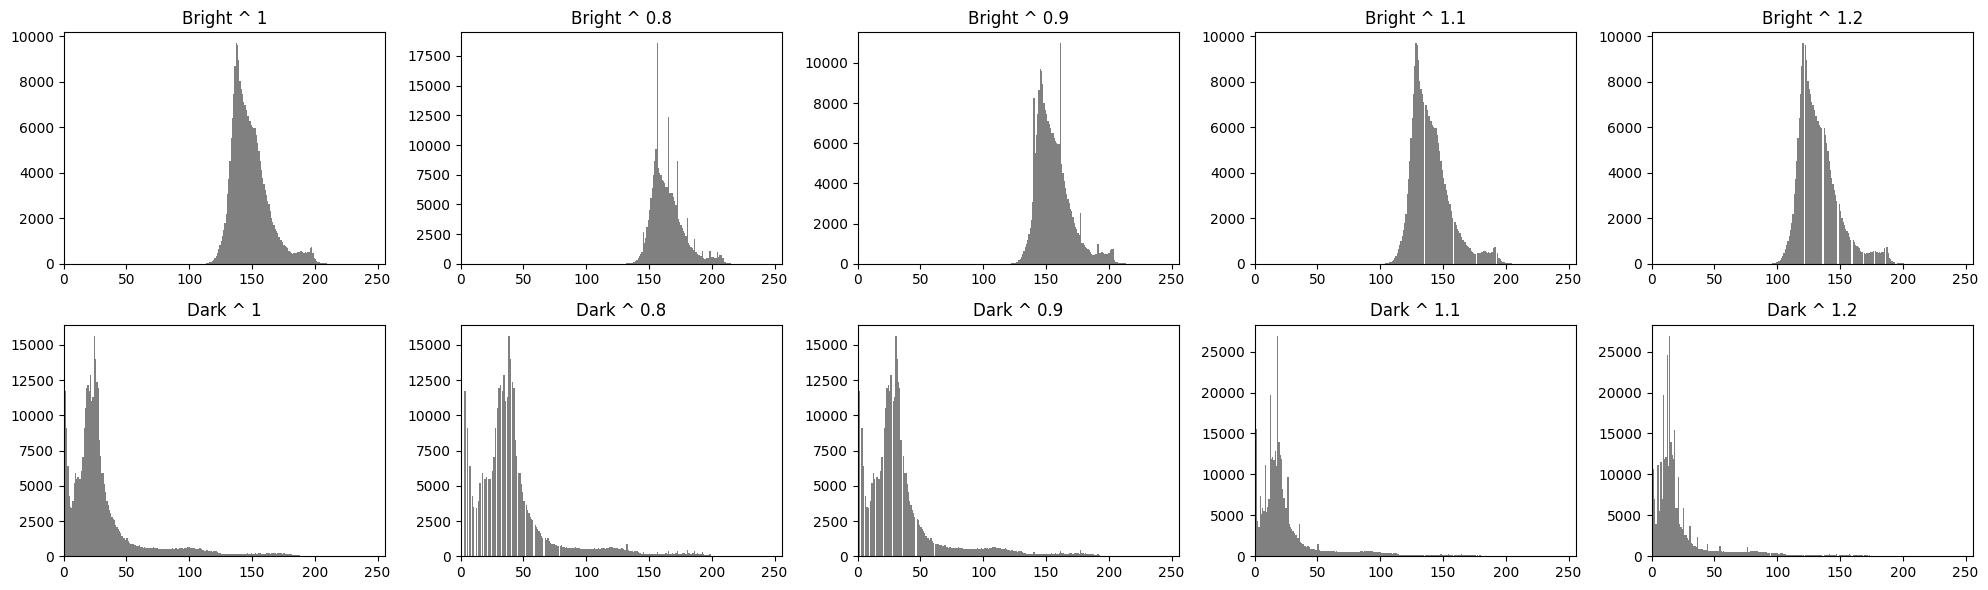
\includegraphics[width=\textwidth]{images/image_24a441.png}
\caption{هیستوگرام تصاویر پس از اعمال صحیح تابع توان. عدم حضور قله‌های مصنوعی در کرانه‌های ۰ و ۲۵۵ نشان‌دهنده حفظ کامل اطلاعات تصویر (\lr{No Clipping}) است.}
\label{fig:gamma_hist_correct}
\end{figure}